\chapter[\csoconeshorttitle{}]{\csoconelongtitle{}}

\label{csoc1}

\beginchapterquote{``Anything is possible if you don't know what you're talking
                     about.''}
                     {Unknown}

%%%%%%%%%%%%%%%%%%%%%%%%%%%%%%%%%%%%%%%%%%%%%%%%%%%%%%%%%%%%%%%%%%%%%%%%%%
%%%%%%%%%%%%%%%%%%%%%%%%%%%%%%%%%%%%%%%%%%%%%%%%%%%%%%%%%%%%%%%%%%%%%%%%%%
%%%%%%%%%%%%%%%%%%%%%%%%%%%%%%%%%%%%%%%%%%%%%%%%%%%%%%%%%%%%%%%%%%%%%%%%%%
\section{Introduction}
%Section tag: INT0
\label{csoc1:sint0}


%%%%%%%%%%%%%%%%%%%%%%%%%%%%%%%%%%%%%%%%%%%%%%%%%%%%%%%%%%%%%%%%%%%%%%%%%%
%%%%%%%%%%%%%%%%%%%%%%%%%%%%%%%%%%%%%%%%%%%%%%%%%%%%%%%%%%%%%%%%%%%%%%%%%%
%%%%%%%%%%%%%%%%%%%%%%%%%%%%%%%%%%%%%%%%%%%%%%%%%%%%%%%%%%%%%%%%%%%%%%%%%%
\section{Potentiometers}
%Section tag: pot0
\label{csoc1:spot0}


%%%%%%%%%%%%%%%%%%%%%%%%%%%%%%%%%%%%%%%%%%%%%%%%%%%%%%%%%%%%%%%%%%%%%%%%%%
%%%%%%%%%%%%%%%%%%%%%%%%%%%%%%%%%%%%%%%%%%%%%%%%%%%%%%%%%%%%%%%%%%%%%%%%%%
%%%%%%%%%%%%%%%%%%%%%%%%%%%%%%%%%%%%%%%%%%%%%%%%%%%%%%%%%%%%%%%%%%%%%%%%%%
\section{Ratiometric Conversion And Measurement Systems}
%Section tag: RCS0
\label{csoc1:srcs0}



%%%%%%%%%%%%%%%%%%%%%%%%%%%%%%%%%%%%%%%%%%%%%%%%%%%%%%%%%%%%%%%%%%%%%%%%%%
%%%%%%%%%%%%%%%%%%%%%%%%%%%%%%%%%%%%%%%%%%%%%%%%%%%%%%%%%%%%%%%%%%%%%%%%%%
%%%%%%%%%%%%%%%%%%%%%%%%%%%%%%%%%%%%%%%%%%%%%%%%%%%%%%%%%%%%%%%%%%%%%%%%%%
\subsection{Introduction}
%Section tag: INT0
\label{csoc1:srcs0:sint0}





%%%%%%%%%%%%%%%%%%%%%%%%%%%%%%%%%%%%%%%%%%%%%%%%%%%%%%%%%%%%%%%%%%%%%%%%%%
%%%%%%%%%%%%%%%%%%%%%%%%%%%%%%%%%%%%%%%%%%%%%%%%%%%%%%%%%%%%%%%%%%%%%%%%%%
%%%%%%%%%%%%%%%%%%%%%%%%%%%%%%%%%%%%%%%%%%%%%%%%%%%%%%%%%%%%%%%%%%%%%%%%%%
\subsection{Observation Error Due To A/D Quantization}
%Subsection tag: OEQ0
\label{csoc1:srcs0:soeq0}

\index{quantization error}
The software which executes on a microcontroller is inherently digital
and can accept as input only digital data.  Analog signals must first be
converted to integers using an \index{A/D converter}A/D converter, and
such a conversion always introduces \index{quantization error}quantization
error as a voltage which is conceptually real is mapped to
$\vworkintsetnonneg{}$.  Any such quantization errors are compounded when
more than one quantized value is used to attempt to infer potentiometer 
position.

The chief emphasis of this section is the analysis of error due to the
use of multiple quantized inputs in an attempt to infer a potentiometer
position.


%%%%%%%%%%%%%%%%%%%%%%%%%%%%%%%%%%%%%%%%%%%%%%%%%%%%%%%%%%%%%%%%%%%%%%%%%%
%%%%%%%%%%%%%%%%%%%%%%%%%%%%%%%%%%%%%%%%%%%%%%%%%%%%%%%%%%%%%%%%%%%%%%%%%%
%%%%%%%%%%%%%%%%%%%%%%%%%%%%%%%%%%%%%%%%%%%%%%%%%%%%%%%%%%%%%%%%%%%%%%%%%%
\subsubsection{Prototype System I}
%Subsubsection tag: OEQ0
\label{csoc1:srcs0:soeq0:spsa0}

In this section we consider the system shown in 
Figure~\ref{fig:csoc1:srcs0:soeq0:spsa0:01}.  
The figure represents
the simplest system which may present quantization
analysis difficulties.  Subsequent sections will analyze
the quantization error of more difficult systems.
Table~\ref{tbl:csoc1:srcs0:soeq0:spsa0:01} defines the
variables used in
Figure~\ref{fig:csoc1:srcs0:soeq0:spsa0:01} and for
analysis in this section.

\begin{figure}
\centering
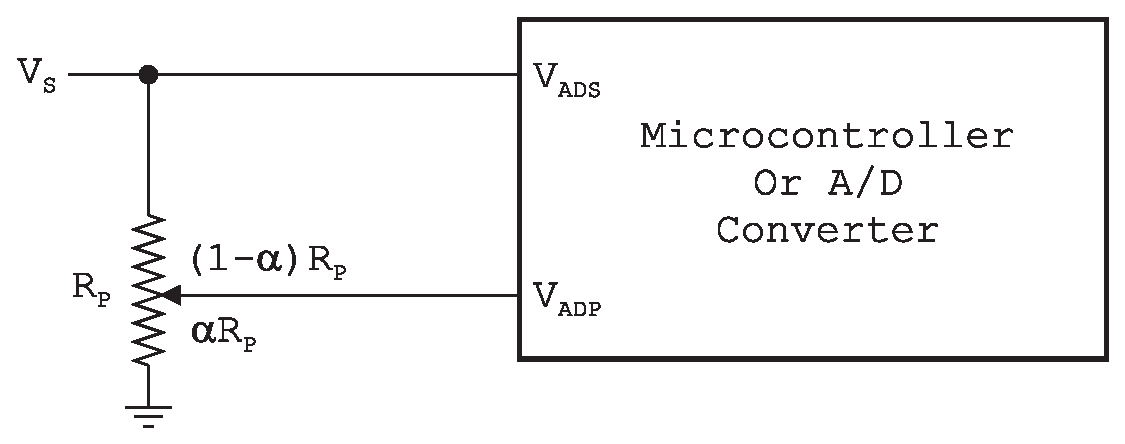
\includegraphics[width=4.6in]{c_soc1/prcs001.eps}
\caption{Prototype Ratiometric Conversion System I}
\label{fig:csoc1:srcs0:soeq0:spsa0:01}
\end{figure}

\begin{table}
\begin{center}
\begin{tabular}{|c|l|}
\hline
Variable           & Description \\
\hline
\hline
$\alpha$           & Potentiometer position, parameterized through $0\leq\alpha\leq 1$. \\
                   & $\alpha=0$ is defined to be the potentiometer position \\
                   & that produces the lowest voltage at the A/D pin, and \\
                   & $\alpha=1$ is defined to be the potentiometer position \\
                   & that produces the highest voltage at the A/D pin.    \\
\hline
$\overline{\alpha}$     
                   & The estimate of potentiometer position, which may    \\
                   & contain error because of quantization error introduced \\
                   & by A/D conversion.                                   \\
\hline
$N_{ADP}$          & The number of A/D counts (supplied to software by an \\
                   & A/D converter) corresponding to the sensing of the   \\
                   & potentiometer position $\alpha$.                     \\
\hline
$\overline{N_{ADP}}$          
                   & $N_{ADP}$ with no quantization error.                \\
\hline
$N_{ADS}$          & The number of A/D counts (supplied to software by an \\
                   & A/D converter) corresponding to the sensing of the   \\
                   & supply voltage $V_S$.                                \\
\hline
$\overline{N_{ADS}}$          
                   & $N_{ADS}$ with no quantization error.                \\
\hline
$R_P$              & The resistance (in Ohms) of the variable potentiometer \\
                   & whose wiper position $\alpha$ is to be sensed (see   \\
                   & Figure~\ref{fig:csoc1:srcs0:soeq0:spsa0:01}).  Note that this resistance does not appear \\
                   & in the analysis of the circuit of Figure~\ref{fig:csoc1:srcs0:soeq0:spsa0:01}, as only  \\
                   & the potentiometer wiper position $\alpha$ affects $V_{ADP}$. \\
\hline
$r_{ADP}$          & The A/D converter ratio (from volts to counts)       \\
                   & implemented by A/D converter monitoring the variable \\
                   & potentiometer input.  Note that $N_P = r_{ADP} V_{ADP}$. \\
\hline
$r_{ADS}$          & The A/D converter ratio (from volts to counts)       \\
                   & implemented by A/D converter monitoring the $V_S$ input. \\
                   & Note that $N_S = r_{ADS} V_{ADS}$.                   \\
\hline
$V_{ADP}$          & The voltage supplied to the microcontroller or A/D   \\
                   & converter corresponding to the variable potentiometer\\
                   & position $\alpha$.  In the system of Figure~\ref{fig:csoc1:srcs0:soeq0:spsa0:01}, $V_{ADP} = \alpha V_S$.\\
\hline
$V_{ADS}$          & The voltage supplied to the microcontroller or A/D   \\
                   & converter corresponding to supply voltage $V_S$.  In \\
                   & the system of Figure~\ref{fig:csoc1:srcs0:soeq0:spsa0:01}, $V_{ADS}=V_S$.  \\
\hline
$V_S$              & The supply voltage, presumed variable, which can be  \\
                   & sensed by the microcontroller software, and also     \\
                   & drives the high side of the variable potentiometer.  \\
\hline
\end{tabular}
\end{center}
\caption{Variables Used In Analysis Of Prototype System I
         (Figure~\ref{fig:csoc1:srcs0:soeq0:spsa0:01})}
\label{tbl:csoc1:srcs0:soeq0:spsa0:01}
\end{table}

To analyze the system depicted in Figure~\ref{fig:csoc1:srcs0:soeq0:spsa0:01},
first note that

\begin{equation}
\label{eq:csoc1:srcs0:soeq0:spsa0:01}
V_{ADS}  =  V_S
\end{equation}

\noindent{}and

\begin{equation}
\label{eq:csoc1:srcs0:soeq0:spsa0:02}
V_{ADP}  =  \alpha V_S.
\end{equation}

For simplicity of analysis, we assume that A/D converters quantize by
truncation, so that

\begin{equation}
\label{eq:csoc1:srcs0:soeq0:spsa0:03}
N_{ADS}  =  \lfloor V_S r_{ADS} \rfloor
\end{equation}

\noindent{}and

\begin{equation}
\label{eq:csoc1:srcs0:soeq0:spsa0:04}
N_{ADP}  =  \lfloor \alpha V_S r_{ADP} \rfloor.
\end{equation}

\noindent{}The assumption that A/D converters quantize by truncation
has little effect on the error analysis of practical systems.  (Need
to include an exercise to show this.)

To aid in symbolic manipulation, we also introduce
$\overline{N_{ADS}}$ and $\overline{N_{ADP}}$, which are
$N_{ADS}$ and $N_{ADP}$, respectively,
without quantization error:

\begin{equation}
\label{eq:csoc1:srcs0:soeq0:spsa0:03b}
\overline{N_{ADS}}  =  V_S r_{ADS}
\end{equation}

\begin{equation}
\label{eq:csoc1:srcs0:soeq0:spsa0:04b}
\overline{N_{ADP}}  =  \alpha V_S r_{ADP}
\end{equation}

If quantization were not present (i.e. if Eqns. 
\ref{eq:csoc1:srcs0:soeq0:spsa0:03}
and 
\ref{eq:csoc1:srcs0:soeq0:spsa0:04}
did not include floor functions), the potentiometer wiper position
$\alpha$ could be calculated exactly as:

\begin{equation}
\label{eq:csoc1:srcs0:soeq0:spsa0:05}
\alpha = \frac{\overline{N_{ADP}} r_{ADS}}{\overline{N_{ADS}} r_{ADP}}.
\end{equation}

Based on (\ref{eq:csoc1:srcs0:soeq0:spsa0:05}),
it makes sense to calculate $\overline{\alpha}$, the
estimate of $\alpha$, as:

\begin{equation}
\label{eq:csoc1:srcs0:soeq0:spsa0:05b}
\overline{\alpha} 
= 
\frac{N_{ADP} r_{ADS}}{N_{ADS} r_{ADP}}.
\end{equation}

The question that must be posed is:
\emph{How different from $\alpha$ can $\overline{\alpha}$ be?}.
We seek to bound $|\overline{\alpha}-\alpha|$.

Quantization can be treated by noting that applying the floor function
to an input introduces an error $\in (-1,0]$, i.e.

\begin{equation}
\label{eq:csoc1:srcs0:soeq0:spsa0:06}
\lfloor x \rfloor = x + \varepsilon; \;\; \varepsilon \in  (-1,0].
\end{equation}

Using this observation, we can rewrite
(\ref{eq:csoc1:srcs0:soeq0:spsa0:05b}) as

\begin{equation}
\label{eq:csoc1:srcs0:soeq0:spsa0:07}
\overline{\alpha} 
= 
\frac{N_{ADP} r_{ADS}}{N_{ADS} r_{ADP}}
=
\frac{(\overline{N_{ADP}} + \varepsilon_1) r_{ADS}}{(\overline{N_{ADS}} + \varepsilon_2) r_{ADP}} ;
\;\;
\varepsilon_1, \varepsilon_2 \in (-1, 0].
\end{equation}

\noindent{}It can be seen from
(\ref{eq:csoc1:srcs0:soeq0:spsa0:07})
that the minimum value of the estimate 
$\overline{\alpha}$ occurs when $\varepsilon_1$ is minimized and 
$\varepsilon_2$ is maximized.  Similarly, the maximum 
value occurs when $\varepsilon_1$ is maximized and 
$\varepsilon_2$ is minimized.  These observations lead to this
inequality:

\begin{equation}
\label{eq:csoc1:srcs0:soeq0:spsa0:08}
\frac{N_{ADP} r_{ADS}}{(N_{ADS}+1) r_{ADP}}
<
\alpha
<
\frac{(N_{ADP}+1) r_{ADS}}{r_{ADP}} .
\end{equation}

Intuitively, the form of (\ref{eq:csoc1:srcs0:soeq0:spsa0:08})
makes sense.  The smallest possible value of $\alpha$ will correspond
to the case
when $N_{ADP}$ contains no quantization error but $N_{ADS}$ contains
a quantization error of nearly 1.
The largest possible value of $\alpha$ will correspond
to the case
when $N_{ADS}$ contains no quantization error but $N_{ADP}$ contains
a quantization error of nearly 1.

It can also be seen from (\ref{eq:csoc1:srcs0:soeq0:spsa0:08}) that
the interval to which $\alpha$ is confined will be larger
when $V_S$ is smaller (implying a smaller $N_{ADS}$ and $N_{ADP}$).
This is also intuitively plausible, since the quantization error 
of up to one count in $N_{ADS}$ or $N_{ADP}$ will have a larger
relative significance when $N_{ADS}$ and $N_{ADP}$ are smaller.

The inequality provided in (\ref{eq:csoc1:srcs0:soeq0:spsa0:08})
is certainly useful, and gives insight into quantization error.  However,
we seek an inequality that is more friendly to engineering work, i.e.
one that involves voltages rather than A/D counts.

Assume it is known for an application that $V_S$ can vary only over the
interval

\begin{equation}
\label{eq:csoc1:srcs0:soeq0:spsa0:08b}
V_S \in [V_{SMIN}, V_{SMAX}], 
\end{equation}


\noindent{}and that $\alpha$ can very only over
the interval 

\begin{equation}
\label{eq:csoc1:srcs0:soeq0:spsa0:08c}
\alpha \in [\alpha_{MIN}, \alpha_{MAX}].
\end{equation}

\noindent{}Furthermore, we
seek useful inequalities where is it \emph{not} required 
that\footnote{(\ref{eq:csoc1:srcs0:soeq0:spsa0:09}) represents the 
requirement that $V_{SMIN}$ or $V_{SMAX}$ represent a precisely 
integral number of A/D
counts.  This requirement is almost never met in practical engineering
work.}

\begin{equation}
\label{eq:csoc1:srcs0:soeq0:spsa0:09}
r_{ADS} \vworkdivides \{V_{SMIN},V_{SMAX}\},
\end{equation}

\noindent{}as if (\ref{eq:csoc1:srcs0:soeq0:spsa0:09})
were required, it would introduce extra complexity 
in applying the inequality.

To develop the desired type of inequality, we can use
a different analysis method.  Assume that 
$r_{ADS}$ and $r_{ADP}$ are fixed.  Then, introduce
the function

\begin{equation}
\label{eq:csoc1:srcs0:soeq0:spsa0:10}
F(\overline{N_{ADP}}, \overline{N_{ADS}}) 
= 
\frac{\overline{N_{ADP}} r_{ADS}}{\overline{N_{ADS}} r_{ADP}},
\end{equation}

\noindent{}which, in accordance with (\ref{eq:csoc1:srcs0:soeq0:spsa0:05}),
is a perfect estimate of $\alpha$.

\begin{figure}
\centering
\Huge{TBD}
\caption{Sample Staircase Pattern Of Estimate $\overline{\alpha}$ Of
         Prototype Ratiometric Conversion System I}
\label{fig:csoc1:srcs0:soeq0:spsa0:02}
\end{figure}

We can examine the staircase pattern of $\overline{\alpha}$ as 
$V_S$ is increased (see Figure \ref{fig:csoc1:srcs0:soeq0:spsa0:02},
which provides an example staircase pattern).  Note that the staircase
pattern may contain four qualitatively
distinct types of vertical discontinuities.  In the descriptions below,
assume that $V_D \in [V_{SMIN}, V_{SMAX}]$ is the value of
$V_S$ at the discontinuity.

\begin{itemize}
\item \textbf{Downward overshoot discontinuities (DOD):}
      As $V_S$ is increased, these correspond to the values
      of $V_S$ where $V_S r_{ADS} \in \vworkintset$ but
      $V_S \alpha r_{ADS} \notin \vworkintset$.  At such 
      discontinuities, 
      $\lim_{V_S \rightarrow V_D^-}\overline{\alpha} > \alpha$,
      but 
      $\lim_{V_S \rightarrow V_D^+}\overline{\alpha} < \alpha$.
\item \textbf{Upward overshoot discontinuities (UOD):}
      As $V_S$ is increased, these correspond to the values
      of $V_S$ where $V_S r_{ADS} \notin \vworkintset$ but
      $V_S \alpha r_{ADS} \in \vworkintset$.  At such 
      discontinuities, 
      $\lim_{V_S \rightarrow V_D^-}\overline{\alpha} < \alpha$,
      but 
      $\lim_{V_S \rightarrow V_D^+}\overline{\alpha} > \alpha$.
\item \textbf{Downward exact discontinuities (DED):}
      As $V_S$ is increased, these correspond to the values
      of $V_S$ where $V_S r_{ADS} \in \vworkintset$ and
      $V_S \alpha r_{ADS} \in \vworkintset$.  At such 
      discontinuities, 
      $\lim_{V_S \rightarrow V_D^-}\overline{\alpha} > \alpha$,
      but 
      $\lim_{V_S \rightarrow V_D^+}\overline{\alpha} = \alpha$.
\item \textbf{Upward exact discontinuities (UED):}
      As $V_S$ is increased, these correspond to the values
      of $V_S$ where $V_S r_{ADS} \in \vworkintset$ and
      $V_S \alpha r_{ADS} \in \vworkintset$.  At such 
      discontinuities, 
      $\lim_{V_S \rightarrow V_D^-}\overline{\alpha} < \alpha$,
      but 
      $\lim_{V_S \rightarrow V_D^+}\overline{\alpha} = \alpha$.
\end{itemize}

We can place upper bounds on the magnitudes of the discontinuities
by examining the partial derivatives of
$F(\overline{N_{ADP}}, \overline{N_{ADS}})$ as specified in
(\ref{eq:csoc1:srcs0:soeq0:spsa0:10}), specifically:

\begin{equation}
\label{eq:csoc1:srcs0:soeq0:spsa0:11}
\frac{\partial{}F(\cdot{},\cdot{})}{\partial \overline{N_{ADS}}}
= 
-
\frac{\overline{N_{ADP}} r_{ADS}}{\overline{N_{ADS}^2} r_{ADP}}
\end{equation}

\begin{equation}
\label{eq:csoc1:srcs0:soeq0:spsa0:11b}
\frac{\partial{}^2 F(\cdot{},\cdot{})}{\partial \overline{N_{ADS}}^2}
= 
2
\frac{\overline{N_{ADP}} r_{ADS}}{\overline{N_{ADS}^3} r_{ADP}}
\end{equation}

\begin{equation}
\label{eq:csoc1:srcs0:soeq0:spsa0:11c}
\frac{\partial{}^i F(\cdot{},\cdot{})}{\partial \overline{N_{ADS}}^i}
= 
(-1)^i (i!)
\frac{\overline{N_{ADP}} r_{ADS}}{\overline{N_{ADS}^{i+1}} r_{ADP}}
\end{equation}


\begin{equation}
\label{eq:csoc1:srcs0:soeq0:spsa0:12}
\frac{\partial{}F(\cdot{},\cdot{})}{\partial \overline{N_{ADP}}}
= 
-
\frac{r_{ADS}}{\overline{N_{ADS}} r_{ADP}}
\end{equation}

\begin{equation}
\label{eq:csoc1:srcs0:soeq0:spsa0:12b}
\frac{\partial{}^i F(\cdot{},\cdot{})}{\partial \overline{N_{ADP}}^i}
= 
0, \; i \geq 2
\end{equation}

A \emph{DOD} (discussed above) corresponds to the case where
$N_{ADS}$ increases by one count at $V_S=V_D$ without an increase in
$N_{ADP}$.    


A \emph{UOD} (discussed above) corresponds to the case where
$N_{ADP}$ increases by one count at $V_S=V_D$ without an increase in
$N_{ADS}$.    




%%%%%%%%%%%%%%%%%%%%%%%%%%%%%%%%%%%%%%%%%%%%%%%%%%%%%%%%%%%%%%%%%%%%%%%%%%
%%%%%%%%%%%%%%%%%%%%%%%%%%%%%%%%%%%%%%%%%%%%%%%%%%%%%%%%%%%%%%%%%%%%%%%%%%
%%%%%%%%%%%%%%%%%%%%%%%%%%%%%%%%%%%%%%%%%%%%%%%%%%%%%%%%%%%%%%%%%%%%%%%%%%
\section{Motion Control Systems}


%End of file c_soc1.tex

